
%(BEGIN_QUESTION)
% Copyright 2008, Tony R. Kuphaldt, released under the Creative Commons Attribution License (v 1.0)
% This means you may do almost anything with this work of mine, so long as you give me proper credit

The following strobe light has a problem: the flash tube never flashes.

$$\includegraphics[width=15.5cm]{i03187x01.eps}$$

Turning the flash rate control (rheostat $R_1$) to the slowest position, you take two voltage measurements with a voltmeter: at test point 3 (between TP3 and ground) you measure a voltage rhythmically pulsating between about 1.5 and 4 volts DC.  At test point 6 (between TP6 and ground) you measure about 0.3 volts DC all the time.

From this information, identify two possible faults (either one of which could account for the problem and all measured values in this circuit), and also identify two circuit elements that could not possibly be to blame (i.e. two things that you know {\it must} be functioning properly, no matter what else may be faulted) other than the 6 volt battery and the on/off switch.  The circuit elements you identify as either possibly faulted or properly functioning can be wires, traces, and connections as well as components.  Be as specific as you can in your answers, identifying both the circuit element and the type of fault.

\medskip
\goodbreak
\item{} Circuit elements that are possibly faulted
\item{1.}
\item{2.} 
\end{itemize}

\medskip
\goodbreak
\item{} Circuit elements that must be functioning properly
\item{1.} 
\item{2.} 
\end{itemize}

\vfil 

\underbar{file i03187}
\eject
%(END_QUESTION)





%(BEGIN_ANSWER)

This is a graded question -- no answers or hints given!

%(END_ANSWER)





%(BEGIN_NOTES)

We know the oscillator section of this circuit is functioning (Q1 -- R1 -- C1) because we see a properly pulsing signal at test point TP3.  However, we do not see a pulsing signal at TP6, which is cause for concern.  Instead, we see what appears to be transistor Q4 turned fully ``on'' and only dropping 0.3 volts between collector and emitter.  

Therefore, we would consider faults anywhere between the output of Q1 and the base of Q4 that could account for Q4 always being turned on.

Another possibility is the primary winding of the transformer failed open, because that would kill any DC path for current to transistor Q4.  Once the capacitor C2 charges up to a value of 5.7 volts (the power supply of 6 volts minus Q4's saturated collector-emitter drop of 0.3 volts), it will hold that voltage value even if Q4 is turning on and off.

\vskip 10pt

Note: the following answers are not exhaustive.  There may be more circuit elements possibly at fault and more circuit elements known to be functioning properly!

\begin{itemize}
\item{} Circuit elements that are possibly faulted
\item{1.} Transistor $Q_2$ failed shorted (collector-to-emitter)
\item{2.} Transistor $Q_3$ failed shorted (collector-to-emitter)
\item{3.} Primary winding of transformer $T_1$ failed open
\item{4.} Resistor $R_4$ failed shorted (possibly -- depends on values of $R_5$ and $R_6$)
\end{itemize}

\begin{itemize}
\item{} Circuit elements that must be functioning properly (besides power supply and signal source)
\item{1.} Rheostat $R_1$
\item{2.} Resistor $R_2$
\item{3.} Capacitor $C_1$
\item{4.} Transistor $Q_1$
\end{itemize}

%INDEX% Troubleshooting review: electric circuits

%(END_NOTES)


